\chapter*{Blog}
        \addcontentsline{toc}{chapter}{Blog}
        \chaptermark{Blog}
	\markboth{Blog}{Blog}
	
	This is the portion of the thesis that I will update regularly with rough notes, lit reviews, results, etc. some of which will be worked in to the real document after some polishing. 
	
	\section{To Do}
	\begin{itemize}
	\item{Obtain flashdrives.     Miguel 9/30/14}
	\item{Set up digital camera.   Miguel 9/30/14}
	\end{itemize}
	
	\subsection{Done}
	\begin{itemize}
	\item{Learn how to use the new \LaTeX\ and Github setup.     Miguel 9/30/14}
	\end{itemize}
	
	\section{Literature Reviews}
	
	    \subsection{Particle-wave association on a fluid interface (Protiere 2006)}
	
	    \subsection{Pilot-Wave Hydrodynamics (Bush 2015)}
	    In this meta-analysis, Bush describes some of the characteristics of the bouncing oil drop experiment that are analagous to effects witnessed in the quantum mechanical world (single-particle diffraction, tunneling, quantized orbits, orbital level splitting, and spin states). Dynamics of the walker are described mathematically. Finally, comparisons to de Broglie's orginal formulation of QM (and not Bohm's) and Stochastic Electrodynamics (?) are made. 
	    \subsubsection{Basic Parameters}
	       Consider a fluid of density $\rho$, viscosity $\nu$, and surface tension $\sigma$, in a bath of depth $H$ driven vertically at an amplitude $A_0$ at frequency $f=\omega/{2\pi}$. By defining $\mathnormal{\gamma}=A_0\omega^2$, the effective gravity in the frame of reference of the bath is $g+\gamma~\mathrm{sin}(\omega t)$. The oil droplet of diameter $D$ bounces in the regime $\gamma<\gamma_F$, where $\gamma_F$ is the Faraday threshold (at this point, Fraday waves appear). The important experimental limits are outlined in Table~\ref{approxlimits}. 
	       
	       	       For certain parameters, the bouncing drop will behave differently. The vibration number describes ``the relative magnitude of the forcing frequency and the drop's natural oscillation frequency," and is given by:
	       	      
\begin{equation} \label{vibrationnumber}
V_i = \frac{\omega}{2}\sqrt{\frac{\rho D^3}{2\sigma}}
\end{equation}   	       	       
	       	       Setting up a plot with $V_i$ on the y axis and $\frac{\gamma}{g}$ on the x axis can help in showing the behavior of the droplet, shown in Fig.~(\ref{regime}). 
	       
	    
	    \begin{figure}[h]
	% the options are h = here, t = top, b = bottom, p = page of figures.
	% you can add an exclamation mark to make it try harder, and multiple
	% options if you have an order of preference, e.g.
	% \begin{figure}[h!tbp]
	   
	       \centering
	    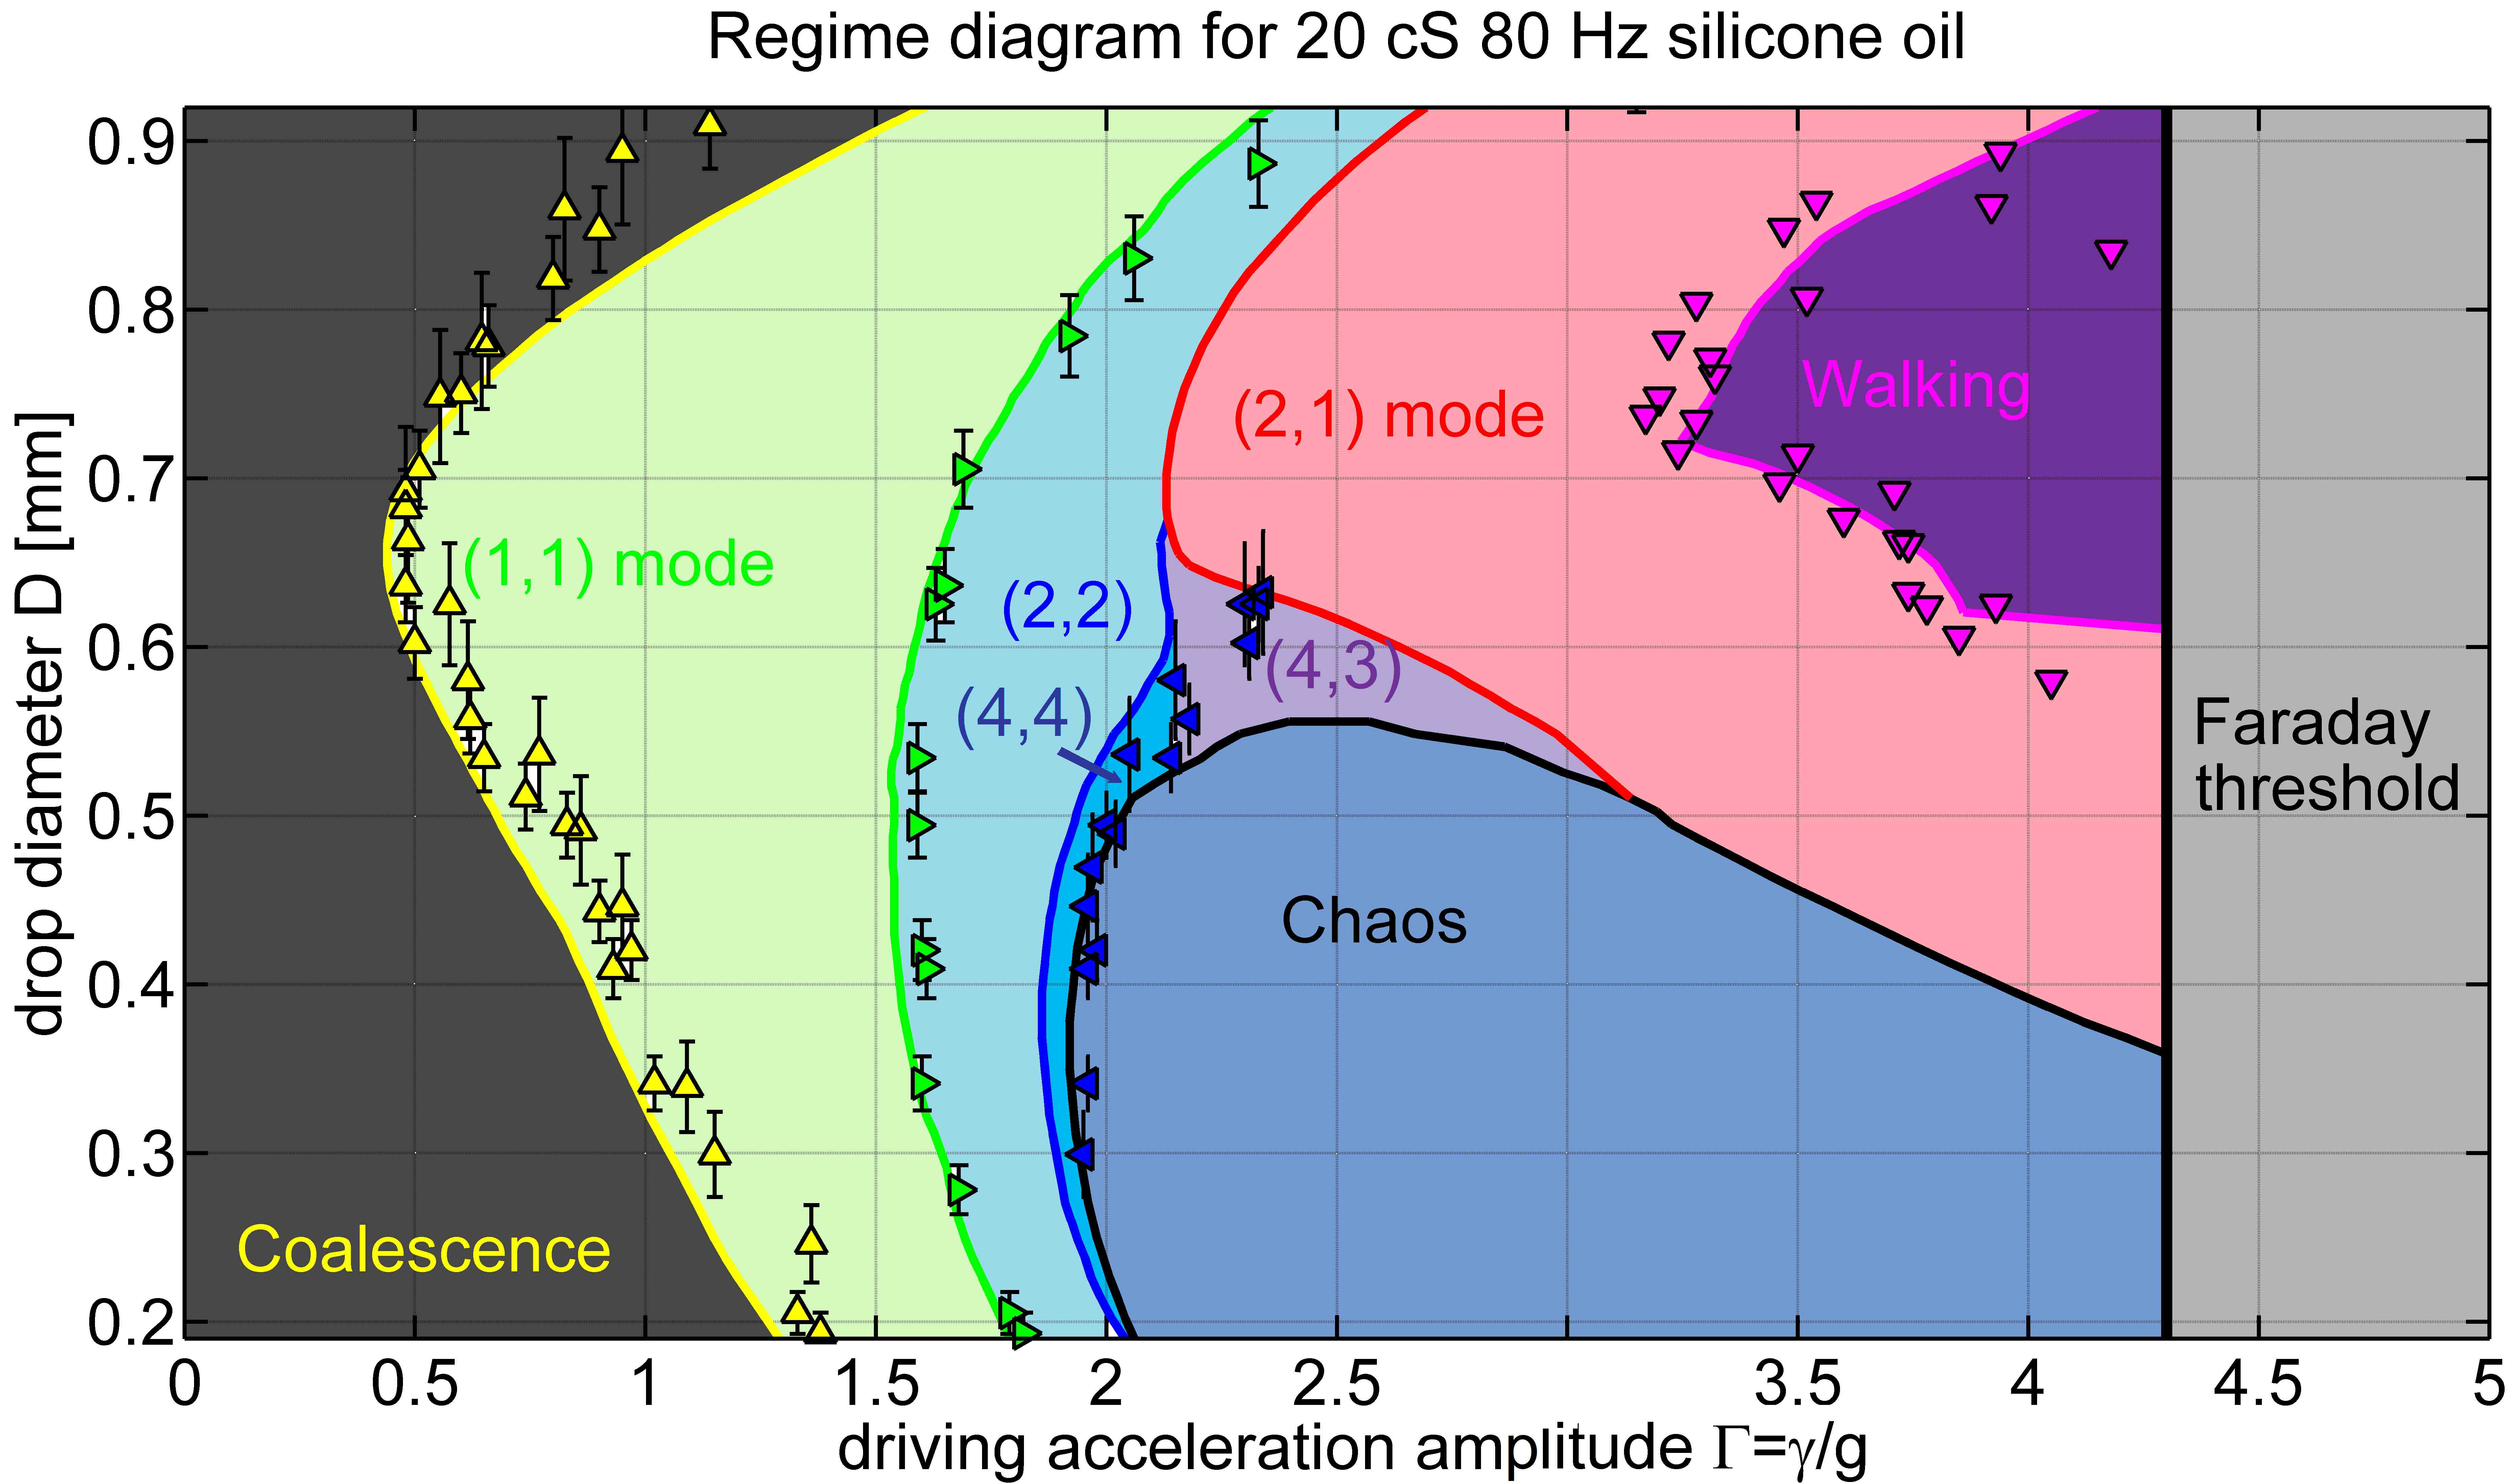
\includegraphics[scale=0.075]{Regime-Mega}
	     \caption{The different bouncing regimes for the oil drops of 20 cS silicon oil and at 80 Hz.}
	 \label{regime}
	\end{figure}

  
	       
	       
\begin{table}[htdp] 
\caption[Basic Table 1]{Approximate Limits for Bouncing Drop Behavior} 
\begin{center} 
\begin{tabular}{c c c} 
\toprule 
  Parameter &  Lower Limit & Upper Limit \\
  \midrule
Viscocity $\nu$ (cSt) & 10 & 100 \\ 
Bath Depth $H$ (mm) & 4 & 10 \\
Frequency $f$ (Hz) & 20 & 150 \\
Amplitude $A_0$ (mm) & 0.1 & 1 \\
Drop Diameter $D$ (mm) & 0.6 & 1.0 \\
\bottomrule 
\end{tabular}
\end{center}
\label{approxlimits} 
\end{table}	\section{Experimental Setup}
	    \subsection{Camera Modification}
